\ifdefined\SingleColumn
\documentclass[10pt,journal,onecolumn,draftclsnofoot]{IEEEtran}
\else
\documentclass[10pt,journal,letterpaper]{IEEEtran}
\fi
\usepackage{amsmath,amssymb,bm,graphicx,booktabs,balance}
\usepackage[hidelinks]{hyperref}
\newcommand{\Fa}{\mathbf F_a}\newcommand{\Fd}{\mathbf F_d}
\newcommand{\pp}{\mathbf p}\newcommand{\xx}{\mathbf x}\newcommand{\ww}{\mathbf w}
\newcommand{\at}{{\mathbf a_t}}\newcommand{\ar}{{\mathbf a_r}}\newcommand{\hh}{\mathbf h}
\newcommand{\norm}[1]{\left\|#1\right\|}
\newcommand{\ALearnGain}{0.00002}
\newcommand{\AFixedMean}{3.50912}
\newcommand{\AFluidMean}{3.50925}
\newcommand{\AFluidLong}{3.50407}
\newcommand{\AClassGain}{0.00065}
\newcommand{\AULARuntimeGap}{0.00067}
\newcommand{\AFluidRuntimeGap}{-0.00010}
\newcommand{\BLearnGain}{0.01022}
\newcommand{\BFixedMean}{2.86862}
\newcommand{\BFluidMean}{3.17039}
\newcommand{\BFluidLong}{3.24819}
\newcommand{\BClassGain}{0.28681}
\newcommand{\BULARuntimeGap}{0.29703}
\newcommand{\BFluidRuntimeGap}{0.02932}
\newcommand{\CLearnGain}{0.00000}
\newcommand{\CFixedMean}{2.57260}
\newcommand{\CFluidMean}{2.81018}
\newcommand{\CFluidLong}{2.93042}
\newcommand{\CClassGain}{0.23840}
\newcommand{\CULARuntimeGap}{0.22472}
\newcommand{\CFluidRuntimeGap}{0.00644}
\newcommand{\ALOS}{3.50952}

\title{L2O Robust Hybrid Beamforming for ISAC with Continuous Fluid Transmit Positioning}
\author{Author names and affiliations to be supplied\thanks{Working research draft, October 2026. The code is an independent implementation. This manuscript has not been submitted.}}
\begin{document}\maketitle
\begin{abstract}
We extend a MinNet--MaxNet learning-to-optimize (L2O) framework to single-user, single-target integrated sensing and communication with continuous fluid transmit positions. Spatial channel reconstruction and an exact spacing projection enable joint training of uncertainty, hybrid-beamforming, receive-filter, and position-update schedules. A controlled study uses independent frozen-design attacks, paired spatial scenarios, and measured online computation. Geometry improves utility in the tested multipath regimes. Coupled L2O provides a modest improvement over its untrained policy without clutter; with clutter, validation retains initialization. These outcomes distinguish geometry benefits from learning benefits and do not establish general learned acceleration or certified robustness.
\end{abstract}
\begin{IEEEkeywords}
Learning to optimize (L2O), algorithm unrolling, fluid antennas, robust hybrid beamforming, integrated sensing and communication.
\end{IEEEkeywords}

\section{Introduction}
Fluid antennas add spatial degrees of freedom to integrated sensing and communication (ISAC), but joint antenna positioning and learning are already established research directions. Fluid-antenna ISAC optimization \cite{zhou}, continuous positioning through deep reinforcement learning \cite{yang}, and generative reinforcement learning for beamforming/port selection \cite{zhang} preclude treating fluid antennas or learned positioning alone as inherently novel.

Wang \emph{et al.}~\cite{wang} develop robust hybrid beamforming by unfolding projected gradient descent--ascent (PGDA) into uncertainty-updating MinNet and beamformer-updating MaxNet stages. We retain these roles and their layer-averaged training loss, specialize the physical model to one user/target, and extend each outer stage with continuous transmit-position updates. Nominal channels are rebuilt from fixed spatial paths, and exact ordered-spacing projection enforces geometric feasibility. The radar receive ULA remains fixed.

The substantive extension under investigation is the \emph{coupled} learning of inherited beamforming/error schedules and new position schedules, rather than learning positions alone. We isolate geometry, learning, and position momentum using fresh paired spatial splits and independent robustness evaluation. The resulting evidence is conditional: the no-clutter multipath case benefits modestly from training, whereas clutter validation retains the untrained policy. The letter therefore reports an implemented extension and its limits, without asserting universal L2O superiority or established publication novelty.

\section{Spatial Hybrid ISAC Model}
\subsection{Geometry and channels}
A narrowband far-field BS has $N_t$ adjustable transmit antennas, $L$ RF chains, and $N_r$ fixed receive antennas. One fixed single-antenna user shares the transmission with one sensing target and $J$ clutter sources. Coordinates are held fixed within each transmission block. For aperture $A$ and minimum separation $d_{\min}$,
\begin{align}
 \mathcal P=\{\pp:\;&0\le p_1,\ p_{n+1}-p_n\ge d_{\min},\nonumber\\
 &n=1,\ldots,N_t-1,\ p_{N_t}\le A\}.\label{eq:P}
\end{align}
Nonemptiness requires $A\ge(N_t-1)d_{\min}$. At wavelength $\lambda$ and broadside angle $\theta$,
\begin{align}
 [\widehat\at(\theta;\pp)]_n&=e^{-j(2\pi/\lambda)p_n\sin\theta},\nonumber\\
 \widehat\hh^H(\pp)&=\sum_{k=1}^{K_c}\beta_k\widehat\at^T(\vartheta_k;\pp).\label{eq:spatial}
\end{align}
The path gains and angles are fixed within a scenario as positions vary. Setting $p_n=(n-1)d$ recovers a ULA under the same spatial channel law. This necessary field-response model replaces the position-independent communication draws in \cite{wang}; old checkpoints are not assumed transferable.

Let $l=0$ denote the target and $l=1,\ldots,J$ clutter. Retaining the reference transpose convention,
\begin{equation}
 \mathbf H_l(\pp)=\alpha_l
 (\widehat\ar_l+\bm\delta_{r,l})
 (\widehat\at_l(\pp)+\bm\delta_{t,l})^T,\quad
 \hh=\widehat\hh+\bm\delta_h.\label{eq:radar}
\end{equation}
Here $\widehat\ar_l$ is the fixed receive-ULA response. The product includes the bilinear perturbation term. Accurate positioning, negligible coupling, and known nominal field parameters are assumed; no physical position-error model is added.

\subsection{Signals, metrics, and robust problem}
Let $\mathbf V=\Fa\Fd=[\mathbf v_c,\mathbf v_s]$, where $\Fd\in\mathbb C^{L\times2}$. Independent unit-power symbols yield covariance $\mathbf V\mathbf V^H$. The user treats the dedicated sensing stream as interference. With $\mathbf q_l=\ww^H\mathbf H_l\mathbf V$,
\begin{align}
 \gamma_c&=\log\left(1+\frac{|\hh^H\mathbf v_c|^2}{|\hh^H\mathbf v_s|^2+\sigma_c^2}\right),\label{eq:comm}\\
 \gamma_s&=\log\left(1+\frac{\norm{\mathbf q_0}_2^2}{\sum_{j=1}^J\norm{\mathbf q_j}_2^2+\sigma_r^2\norm{\ww}_2^2}\right).\label{eq:sense}
\end{align}
Both streams illuminate the target. The inherited sensing MI surrogate sums clutter powers, assuming negligible effective echo cross-correlations. Independent transmit symbols alone do not remove coherent echo cross terms. Neither this metric nor the experiments measure detection/estimation accuracy. Natural logarithms give the communication metric in nats/s/Hz. There is no inter-user interference or SIC.

The unchanged uncertainty balls are
\begin{equation}
 \norm{\bm\delta_h}_2\le\epsilon_h\sqrt{N_t},\quad
 \norm{\bm\delta_{t,l}}_2\le\epsilon_t\sqrt{N_t},\quad
 \norm{\bm\delta_{r,l}}_2\le\epsilon_r\sqrt{N_r}.\label{eq:balls}
\end{equation}
Writing their product sets as $\mathcal A_h,\mathcal A_t,\mathcal A_r$, the objective is
\begin{equation}
\begin{aligned}
 \max_{\pp,\Fa,\Fd,\ww}\quad&\rho\min_{\mathcal A_h}\gamma_c+
 (1-\rho)\min_{\mathcal A_t\times\mathcal A_r}\gamma_s\\
 \mathrm{s.t.}\quad&\pp\in\mathcal P,\quad |[\Fa]_{n\ell}|=1,\\
 &\norm{\Fa\Fd}_F^2=P,\qquad\norm{\ww}_2^2=1.
\end{aligned}\label{eq:problem}
\end{equation}
Separate error blocks permit the two minima. Common radii are retained across geometries; they are unstructured response errors rather than one common angle error. A weighted objective does not impose minimum task-specific QoS.

\section{Fluid-Position MinNet--MaxNet Unrolling}
\subsection{Inherited and added update blocks}
Let $u=\rho\gamma_c+(1-\rho)\gamma_s$ and $b=(\Fa,\Fd,\ww)$. At layer $k$, rebuild spatial channels from $\xx^k=\pp^k/\lambda$. MinNet simultaneously updates the three error blocks by descending their respective communication or sensing metrics, adding momentum, and projecting their balls. MaxNet reevaluates gradients at the updated errors and old beamformers, then simultaneously ascends the three beamforming/filter blocks using $u$, with momentum. These are the inherited equations (11)--(16) of \cite{wang}.

Analog entries are mapped to unit phases; digital weights are normalized using the \emph{updated} analog matrix to enforce effective power; receive filters are normalized. Existing deterministic fallbacks handle zero proposals. These mappings enforce feasibility without claiming joint Euclidean projection onto the nonconvex hybrid set.

The new position block follows those stages sequentially:
\begin{align}
 \widetilde\xx^{k+1}&=\xx^k+\mu_p^k\nabla_{\xx}u
       +\eta_p^k(\xx^k-\xx^{k-1}),\nonumber\\
 \xx^{k+1}&=\Pi_{\mathcal X}(\widetilde\xx^{k+1}),\quad
 \mathcal X=\{\xx:\lambda\xx\in\mathcal P\}.\label{eq:position}
\end{align}
The partial is evaluated at current positions and newly updated errors/beamformers, holding those variables fixed. From \eqref{eq:spatial},
\begin{equation}
 \frac{\partial\widehat a_{t,l,n}}{\partial x_n}
 =-j2\pi\sin\theta_l\widehat a_{t,l,n}.\label{eq:derivative}
\end{equation}
For stored $\widehat h_n$, conjugate the corresponding path sum. With inherited Wirtinger derivatives $g_h=\partial\gamma_c/\partial\hh^*$ and $g_{t,l}=\partial\gamma_s/\partial\at_l^*$,
\begin{equation}
 [\nabla_{\xx}u]_n=2\Re\left\{\rho g_{h,n}^*\frac{\partial\widehat h_n}{\partial x_n}
 +(1-\rho)\sum_{l=0}^{J}g_{t,l,n}^*\frac{\partial\widehat a_{t,l,n}}{\partial x_n}\right\}.\label{eq:chain}
\end{equation}
This incorporates both utility components and full perturbed radar channels. It is not the exact derivative of an unknown globally minimized robust value. Physical-position derivatives divide by $\lambda$.

For $a=A/\lambda$ and $d=d_{\min}/\lambda$, exact Euclidean projection of $\mathbf y$ solves
\begin{equation}
 \min_{0\le z_1\le\cdots\le z_{N_t}\le a-(N_t-1)d}
 \sum_n[z_n-y_n+(n-1)d]^2,\label{eq:pav}
\end{equation}
then restores $x_n=z_n+(n-1)d$. Bounded isotonic regression via pool-adjacent-violators gives an $O(N_t)$ construction. Its exact active-face Jacobian averages gradients on free pooled blocks and vanishes on clamped blocks, away from transitions. No straight-through approximation is used.

\subsection{Coupled training and controls}
For $K$ layers, train the six inherited step/momentum pairs plus $(\mu_p^k,\eta_p^k)$: $14K$ scalar parameters. The fixed-array model has $12K$; fixing position momentum leaves $13K$ active fluid parameters. Initial position momentum is zero. No EpsNet or RecNet is enabled, and no configuration generalization is asserted.

We retain the direct unconstrained coefficient parameterization and the inherited loss
\begin{equation}
 \mathcal L=-\frac{1}{K|\mathcal D|}
 \sum_{i\in\mathcal D}\sum_{k=1}^{K}u_i^k.\label{eq:loss}
\end{equation}
Full differentiation passes through uncertainty, beamforming, spatial, momentum, and projection operations. Error iterates are not detached. Both MinNet and MaxNet schedules are updated by the same joint training loss, as in the inherited procedure; this is not an independent adversarial training objective. Accordingly, independent attacks remain essential when assessing learned robustness.

The classical fluid control uses zero position momentum and up to six fixed-error Armijo trials with step halvings. The unfolded policy uses its learned direct update without backtracking. An untrained policy with the same no-backtracking architecture isolates learning from this overhead difference. A full analytic helper call computes all six inherited gradient blocks: fixed layers use two calls, fluid layers three. Equal calls are not equal FLOPs.

\begin{figure*}[t]\centering
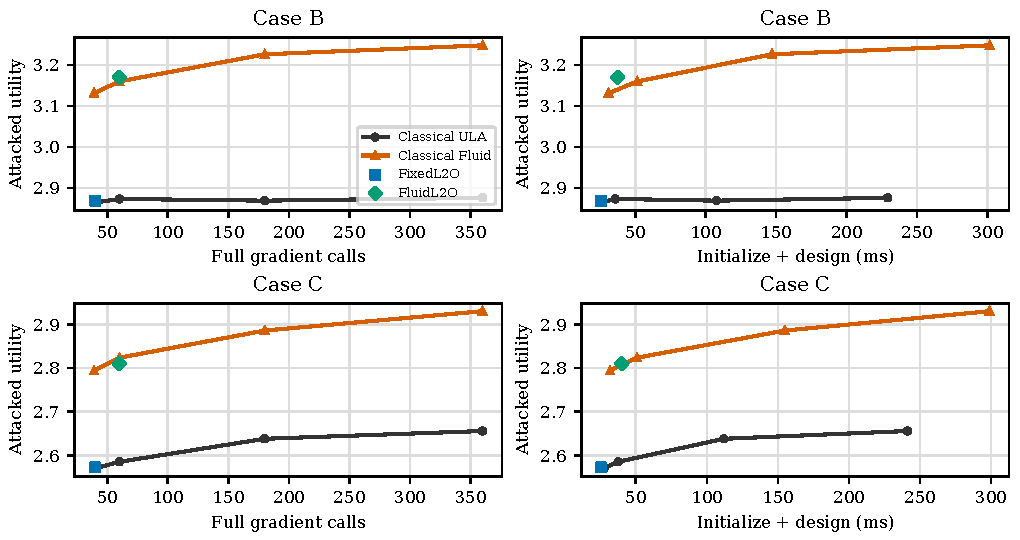
\includegraphics[width=.96\textwidth]{figures/compute.pdf}
\caption{Measured design computation and independent attack evaluation on100 paired scenarios per regime. Learned points average three runs. Classical curves include separately retuned fixed-ULA budgets and longer fluid solves; gradient counts are full six-block helper calls. Runtime includes initialization and the complete online design call.}\label{fig:compute}
\end{figure*}

\section{Controlled Numerical Study}
\subsection{Scenarios, training, and evaluation}
We use $N_t=N_r=8$, $L=4$, $A=3.5\lambda$, $d_{\min}=0.25\lambda$, a fixed half-wavelength receive ULA, $\rho=0.8$, unit noise variances, $P=10^{5/10}$, and $\epsilon_h=\epsilon_t=\epsilon_r=0.05$. All methods have common aperture, antenna/RF counts, power, paths, and error sets. The fixed ULA has half-wavelength spacing; $\lambda=0.01$ m only converts units.

Each regime has fresh disjoint 128/32/100 train/validation/test scenarios. A is aligned unit-magnitude LOS with no clutter. B/C use four fixed complex Gaussian communication path gains, normalized variances proportional to $(0.75^2,0.4^2,0.4^2,0.4^2)$, dominant departure angle in $[-30^\circ,-20^\circ]$, and other angles in $[-65^\circ,65^\circ]$. Target angles lie in $[25^\circ,35^\circ]$ for B and $[20^\circ,30^\circ]$ for C. C adds one clutter source $8^\circ$--$12^\circ$ beyond the target. Gaussian target/clutter reflection variances are 2/3 dB. Gains/angles never change during position optimization.

Classical scalar steps are selected by validation-only grids. Fixed-array settings are retuned at each gradient budget. Fluid uses the 20-iteration ULA beamforming settings and tunes position steps per budget. Learned models start from a validation-tuned no-backtracking scalar initialization, without transferring old checkpoints. Initialization uses nominal channel phases and target matching, with 90/10 communication/sensing power allocation in B/C and 100/0 in A.

At $K=20$, SGD uses learning rate $10^{-4}$, decay $0.98$, batch size 32, and ten epochs (40 updates). Three paired shuffle seeds train each primary fixed/fluid model; the zero-position-momentum ablation uses one seed. Validation selects the lowest inherited layer loss, including epoch 0. Independently attacked validation is logged but does not silently replace the loss or selection rule. Additional controls include a single fixed random geometry and a common geometry fitted on training scenarios then frozen at test time.

Final evaluation freezes positions and beamformers. It uses zero/terminal errors, five random feasible starts, 50 projected-Adam steps, and nested 50/200/1000-step projected-gradient searches with best-so-far retention. Communication and sensing errors are searched consistently with the separate minima. All methods receive a shared feasible uncertainty pool evaluated on each recipient's frozen geometry and beamformers. Reported values are lowest utilities found, upper bounds on the unknown robust minima. They are not global certificates. Raw states, attacks, per-scenario metrics, residuals, costs, and source hashes are retained.

\begin{table}[t]\centering\footnotesize
\caption{Independently attacked utility at 20 iterations/layers. L2O means average three paired runs.}\label{tab:main}
\setlength{\tabcolsep}{3pt}
\begin{tabular}{ccccc}\toprule
Case & Classical ULA & Fixed L2O & Classical fluid & Fluid L2O\\\midrule
A & 3.50908 & 3.50912 & 3.50923 & 3.50925 \\
B & 2.86458 & 2.86862 & 3.16017 & 3.17039 \\
C & 2.57044 & 2.57260 & 2.82386 & 2.81018 \\
\bottomrule

\end{tabular}
\par\smallskip\scriptsize Fixed designs use40 full gradient calls; fluid designs60. Runtime comparisons are shown separately.
\end{table}

\subsection{What geometry and learning each contribute}
Table~\ref{tab:main} separates fixed-array learning from fluid extension. At 60 full calls, classical geometry gains over ULA are $\BClassGain$ in B and $\CClassGain$ in C. These are geometry/optimization gains, not learning gains. The coupled fluid model achieves $\BFluidMean$ in B and $\CFluidMean$ in C. Its comparison with the identical untrained policy is given in Table~\ref{tab:learning}.

\begin{table}[t]\centering\footnotesize
\caption{Learning effect at matched architecture/depth: trained fluid minus untrained fluid. Paired intervals resample 100 scenarios after averaging runs.}\label{tab:learning}
\setlength{\tabcolsep}{3pt}
\begin{tabular}{cccc}\toprule
Case & Untrained & Trained & Difference95\% interval\\\midrule
A & 3.50923 & 3.50925 & $[1.73,2.31]\times10^{-5}$ \\
B & 3.16017 & 3.17039 & [+0.00850, +0.01195] \\
C & 2.81018 & 2.81018 & $[-2.38,1.43]\times10^{-8}$ \\
\bottomrule

\end{tabular}
\end{table}

The B gain is $\BLearnGain$, modest relative to the geometry gain. In C, all fluid seeds select epoch 0, so the observed $\CLearnGain$ training gain is zero. Training attempts and unfavorable selections remain in the accounting. The momentum ablation has one seed and shows no practically material benefit in this pilot; it cannot support a broad conclusion about position momentum.

In aligned LOS, an MRT transmit vector, zero dedicated sensing power, and matched receive filter attain the geometry-independent robust optimum
\begin{align}
 U_{\rm LOS}={}&\rho\log(1+PN_t(1-\epsilon_h)^2/\sigma_c^2)\nonumber\\
 &+(1-\rho)\log(1+S_s(1-\epsilon_t)^2(1-\epsilon_r)^2),\label{eq:los}
\end{align}
where $S_s=|\alpha_0|^2PN_tN_r/\sigma_r^2$. Cauchy--Schwarz bounds and opposing ball errors attain these factors, independent of feasible positions. The analytic ULA control averages $\ALOS$. Finite optimizer drift relative to that control must not be interpreted as an intrinsic geometry benefit. This closed form is limited to the stated LOS regime.



\subsection{Runtime, components, and feasibility}
Figure~\ref{fig:compute} compares gradient budgets and actual online runtime. Longer classical fluid solves reach $\BFluidLong$ in B and $\CFluidLong$ in C; the short learner does not establish superiority over those attainable values. Validation timing selects nearby classical iteration budgets. Relative to that fluid runtime control, the learned gaps are $\BFluidRuntimeGap$ and $\CFluidRuntimeGap$ in B/C. These are approximate runtime matches, not equal deadlines; actual times are retained.

\begin{table}[t]\centering\footnotesize
\caption{Learned components and online median/p95 ms, averaged across paired runs.}\label{tab:components}
\begin{tabular}{cccc}\toprule
Case/array & Communication & Sensing metric & Time\\\midrule
B/Fixed & 2.7137 & 3.4882 & 25.7/28.3 \\
B/Fluid & 3.0141 & 3.7957 & 37.7/43.0 \\
C/Fixed & 2.6425 & 2.2931 & 25.5/28.8 \\
C/Fluid & 2.8587 & 2.6160 & 40.1/43.2 \\
\bottomrule

\end{tabular}
\end{table}

Timing uses one AMD EPYC9V74 CPU thread, complex64/float32, batch one, three warmups, and three repeats on 20 test scenarios. It includes initial beamformer construction, coefficient access, spatial reconstruction, gradients, projections, layer metrics, and classical backtracking. Offline fitting and independent attack time are recorded separately. CSI acquisition, antenna movement/settling, and RF programming are unmodeled; no sub-millisecond hardware claim follows.

Feasibility checks cover analog modulus, effective power, receive norm, uncertainty balls, aperture, and spacing. Tests include independent signal calculations, float64 position/full-unroll finite differences, tiny independent projection QPs, fixed-array equivalence, frozen-variable checks, and recipient-scored attack-pool regression. Independent NumPy checks and complete source replay verify saved results. Numerical feasibility does not certify a global robust optimum. Task components in Table~\ref{tab:components} remain necessary because weighted utility alone does not guarantee improvement in both tasks.


\section{Conclusion}
The inherited MinNet--MaxNet framework can be extended with spatial reconstruction and exact spacing-projected fluid-position updates, jointly learning all update schedules. Controlled results support geometry gains and a modest no-clutter learning gain, but the inherited training/selection procedure yields no clutter learning gain. These limits motivate stronger training studies and matched competing baselines before claims of general acceleration, novelty, or practical deployment.

\noindent\emph{Artifacts:} \url{https://github.com/muneefo/L2O_ISAC}, under \path{experiments/fluid_tx_l2o/}. This is an independent reconstruction/extension, not author-released software.
\begin{thebibliography}{4}
\bibitem{zhou} L. Zhou, J. Yao, M. Jin, T. Wu, and K.-K. Wong, ``Fluid antenna-assisted ISAC systems,'' \emph{IEEE Wireless Commun. Lett.}, vol.13, no.12, pp.3533--3537, 2024, doi:10.1109/LWC.2024.3476148.
\bibitem{yang} S. Yang \emph{et al.}, ``Towards intelligent antenna positioning: Leveraging DRL for FAS-aided ISAC systems,'' arXiv:2501.01281, 2025.
\bibitem{zhang} J. Zhang \emph{et al.}, ``Generative reinforcement learning for fluid antenna systems based sensing and communication,'' \emph{npj Wireless Technology}, vol.2, Art.30, 2026, doi:10.1038/s44459-026-00035-0.
\bibitem{wang} L. Wang, S. A. Vorobyov, and E. Ollila, ``L2O robust hybrid beamforming for ISAC,'' \emph{IEEE Trans. Wireless Commun.}, vol.25, pp.18778--18794, 2026, doi:10.1109/TWC.2026.3702925.
\end{thebibliography}\end{document}
